\section{Introduction}

Agilefant is an open source tool for agile project management. Currently it is
provided as an open-source version and a hosted version. The hosted version
comprises more features in comparison to the open-source version.

Agilefant has approximately 10,000 users worldwide, and according to the
customer, the number of registered users increases every day.
 
Agilefant is a very powerful tool for requirement management but currently it is
too detailed to be used on mobile devices (small screens). The customer wishes
that the users of Agilefant could use its the most important functions using
their mobile phones and tablets. For example, users could log spent hours after
a workday when sitting in a bus. Agilefant's main competitors are already
providing mobile applications, so it is crucial to Agilefant to also provide a
mobile client. Therefore, the goal of our group is to develop a mobile
application that works along the hosted version of Agilefant and can be used on
both smart phones and tablets.

\subsection{Vision}

Customer's vision is to become the leading provider of agile backlog management
tools. This mobile application has an important role of fulfilling the vision as
missing mobile support can be a major threshold factor for many potential
new users.

\section{Stakeholders and staffing}

The project contains several stakeholders, which are presented in
Figure~\ref{fig:stakeholders}. The stakeholders are divided into four main
groups: the customer (Agilefant), the student group, the teaching personnel in
Aalto University, and teaching personnel in University of Victoria (UVic).
In addition to these, Amazon's web server is listed as a stakeholder as the
application needs to communicate with it. Arrows in the figure present the
direction of main communication. 

\begin{figure}[H]
\centering
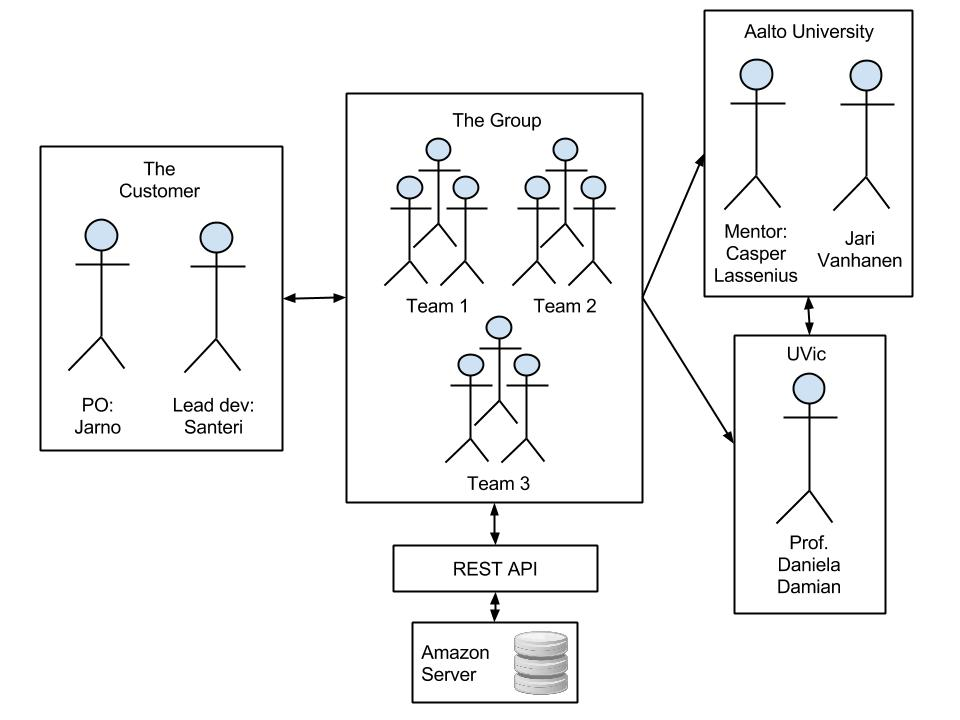
\includegraphics[width=1\textwidth]{imgs/stakeholders.jpg}
\caption{Stakeholders of the project}
\label{fig:stakeholders}
\end{figure}

\subsection{The Team}

At the beginning of the course we had a team of 9 people, but we lost one
developer so now we have only 8 students. At the beginning of 2014, 15 Canadian
students will join us, so we will have a group of 23 students. We will form
three teams, each of them consisting of both Finns and Canadians.

In this document, only some personal information is published. We have a
document with stakeholders' more detailed personal information but we don't
want to make that public.

The group's webpage is
\href{https://github.com/phyper/mobilefant-documentation/wiki}{https://github.com/phyper/mobilefant-documentation/wiki}
and its email is mobilefant\#mobilefant.flowdock.com.

We have several roles and one person can have several roles. The primary role
given by the course is bolded. The roles are:

\begin{itemize}
  \item Project Manager = PM
  \item Scrum Master = SM
  \item Lead Architect = AR
  \item Quality Assurance = QA
  \item Requirements Engineering = RE
  \item Developer = Dev
\end{itemize}

\begin{table}[H]
\center
\resizebox{\textwidth}{!}{
\begin{tabular}{|p{1.8cm}|p{3cm}|p{4.1cm}|p{4.1cm}|p{1.8cm}|} 
	
\hline % The line on top of the table
\textbf{Role} & \textbf{Name} & \textbf{Email} & \textbf{Responsibilities} & 
\textbf{Assistant role} \\ 
\hline 
\textbf{PM}, SM, RE & Benjamin Behm & benjamin.behm\#aalto.fi & Organizing the 
work, removing impediments, documentation, process supervising, eliciting 
requirements, working as a scrum master & - \\ 
\hline
\textbf{AR}, RE & Harri Lampi & harri.lampi\#aalto.fi & Architectural design, 
eliciting requirements, coding, UI design, documentation & - \\ 
\hline
\textbf{QA}, RE & Matias Kuusela & matias.kuusela\#aalto.fi & Quality assurance,
eliciting requirements, UI design, documentation & -\\ 
\hline
\textbf{Dev} & Miro Vilkki & miro.vilkki\#aalto.fi & End-to-end development & AR\\
\hline
\textbf{Dev} & Rolle Saarinen & rolle.saarinen\#aalto.fi & End-to-end
development & AR\\
\hline
\textbf{Dev} & Janne Gröndahl & janne.grondahl\#aalto.fi & End-to-end
development & QA\\
\hline
\textbf{Dev} & Janne Kajovuori & janne.kajovuori\#aalto.fi & End-to-end
development, documentation, UI design & PM\\
\hline
\textbf{Dev} & Joakim Kronqvist & joakim.kronqvist\#aalto.fi & End-to-end
development & AR\\
\hline

\end{tabular}
}
\caption{The Finns}
\label{table:Team}
\end{table}

\subsection{Mentor}

\begin{table}[H]
\center
\begin{tabular}{|p{2cm}|p{3.8cm}|p{4.1cm}|} 

\hline 
\textbf{Role} & \textbf{Name} & \textbf{Email} \\ 
\hline
Mentor & Casper Lassenius & casper.lassenius\#aalto.fi \\
\hline
\end{tabular}
\caption{Mentor in Finland}
\label{table:Mentor}
\end{table}

\subsection{Customer}

\begin{table}[H]
\center
\begin{tabular}{|p{2cm}|p{3.8cm}|p{4.1cm}|} 
	
\hline 
\textbf{Role} & \textbf{Name} & \textbf{Email}\\ 
\hline
Product owner & Jarno Vähäniitty & jarno\#agilefant.org\\
\hline
Tech. Lead & Santeri Korri & santeri\#agilefant.org\\
\hline
\end{tabular} 
\caption{Customer representatives}
\label{table:Customer}
\end{table}

\subsection{Teaching personnel in UVic}

\begin{table}[H]
\center
\begin{tabular}{|p{2cm}|p{3.8cm}|p{4.1cm}|} 
	
\hline 
\textbf{Role} & \textbf{Name} & \textbf{Email}\\ 
\hline
Professor & Daniela Damian & damian.daniela\#gmail.com\\
\hline
\end{tabular} 
\caption{Staff in University of Victoria}
\label{table:Customer}
\end{table}



\section{The Goals}
\subsection{Project goals}

The main goal is to develop a reliable mobile application for Agilefant that
contains  the main functionalities of its cloud version and fulfil customer's
vision of  the product. Furthermore, the goal is that everyone's personal goals
will be reached and the course has been an educational experience. Other high
level goals are identified, and these are presented in
Table~\ref{table:Projectgoals}.

\begin{table}[H]
\center
\resizebox{\textwidth}{!}{
\begin{tabular}{|p{0.5cm}|p{6cm}|p{7cm}|} 

\hline 
\centering \textbf{\#} & \textbf{Goal} & \textbf{Verification Criteria} \\ 
\hline

\centering 1 & To produce high customer satisfaction & Customer's personal
opinion about the delivered product. \\
\hline

\centering 2 & To implement a limited set of key use cases & Architecturally
sound, clear implementation and testable. \\
\hline

\centering 3 & The product will be released after the project & Whether the
customer release the product or not. \\ 
\hline

\centering 4 & To produce an application that is easy to develop further &
The customer's developers understand the code easily and they have no
difficulties to add new features in it. \\
\hline


\centering 5 & To get grade 5 & The grade will be visible in transcript of
records or the course personnel has verified the grade. \\ 
\hline

\centering 6 & To win the quality award & Our group has selected as the best
group at the end of the course. \\ 
\hline

\end{tabular}
}
\caption{Project goals in a priority order}
\label{table:Projectgoals}
\end{table}


\subsection{Personal learning goals}

As we are here learning new things, we should focus on to learn things we are
interested in. Thus, it is important that everyone tells theirs interests aloud
and points out what they would like to learn during this course. In this reason,
everyone has written down their
\href{https://docs.google.com/spreadsheet/ccc?key=0Ahu59q_GwtcedHJZdjQ1RWROZFYxa0RTcWp3MkJkTnc&usp=sharing}{personal learning goals}. To reach these
goals, people should try to participate in tasks that support their learning
goals. If a developer is going to take this course second time later and has a
preferable role in his mind, it is really recommendable that he helps that SE
trio's member.

\section{Resources}
\subsection{Personnel}

The course in Finland is a course of fixed hours, meaning that the
Finns must invest ``credits * 27 hours - 15 hours'' in the project. For example
a person with 8 credits must spend 201 hours during the project.

In Figure~\ref{fig:timeallocation}, we have estimated hours everyone is going to
use during the course. The same information is available in a
\href{https://docs.google.com/spreadsheet/ccc?key=0Ahu59q_GwtcedHI3MnJQM0NWZS11aGxFTzFZeVEyQVE&usp=sharing}{time allocation spreadsheet}. In that spreadsheet we
also follow how much effort has been used and how much is left.

\begin{figure}[H]
\centering
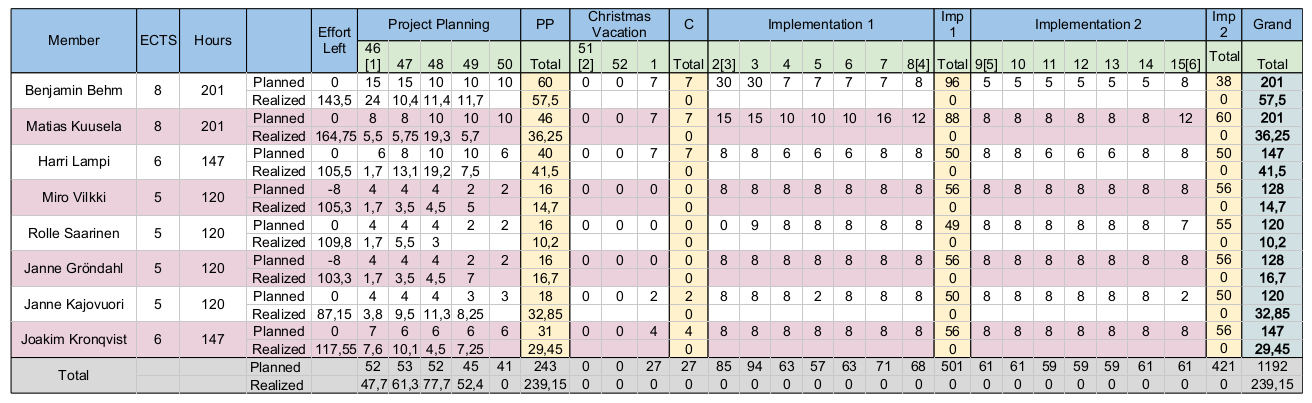
\includegraphics[width=1\textwidth]{imgs/timeallocation.png}
\caption{Time allocation (updated on 2013/12/06)}
\label{fig:timeallocation}
\end{figure}

In a Figure~\ref{fig:hours_phases}, it can be seen that total hours used in the
planning phase is almost equivalent with the planned hours. The figure doesn't
count hours used in the last week of the planning phase.

\begin{figure}[H]
\centering
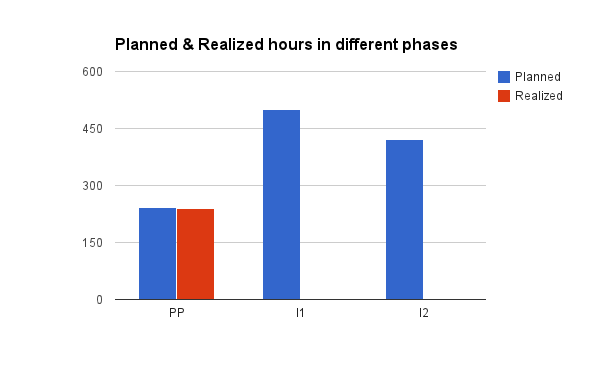
\includegraphics[width=1\textwidth]{imgs/chart_1.png}
\caption{Hours per a phase (updated on 2013/12/06)}
\label{fig:hours_phases}
\end{figure}

Figure~\ref{fig:hours_weeks} shows the planned and realized hours a weekly
basis. It is clearly visible that after the first week the realized hours
exceeded the planned hours. The Finns should monitor used hours to be sure that
hours won't run out in the middle of the course. The project manager monitors
regularly the spent effort.

\begin{figure}[H]
\centering
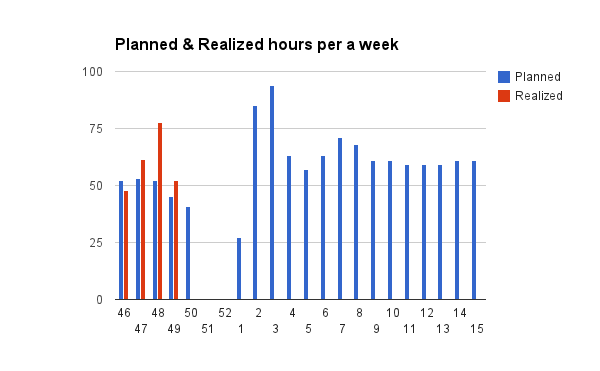
\includegraphics[width=1\textwidth]{imgs/chart_2.png}
\caption{Hours per a week}
\label{fig:hours_weeks}
\end{figure}

Hour estimates will be adjusted again at the beginning of Sprint 3 when students
know their spring's schedule and we get more information about Canada
cooperation.

\subsection{Material}

\paragraph{Development tools}~

Development tools used during the course are IntelliJ IDEA 12
Ultimate, Apache Cordova, Android SDK, XCode (on Mac), and Github. The project
manager has a JetBrain's Classroom License so IntelliJ's full version can be
used.

\paragraph{Communication tools}~

Flowdock is used as a primary communication tool. Aalto provides 180 days
license for that. Google Hangout will be used as a video conferencing tool.

\paragraph{Design tools}~

Lucidchart tool is used to draw UI wireframes and other diagrams.

\paragraph{Working space}~

Development will take place at CS building in the room A243. The room is shared
with an another project group (\#15 - TrafficSense) so we have been scheduled
the usage of the room with them. The idea will be that the both teams will have
specific days and hours the room is exclusively reserved for them. At other
times, everyone could use the room. Currently we have agreed that our team uses
the room on Monday and Thursday, and the another team on Friday and Tuesday or
Wednesday. We have shared our calendar with them so they know when the room is
available.

The CSE department borrowed three desktop computers to our group with Ubuntu
12.04 installed. These computers have been set up to our team room.

\paragraph{Testing devices}~

We need mobile devices to test the application. The customer has promised to
deliver some test devices, but the selection will be limited. In this reason we
will also use our own mobile phones for testing. We have phones with IOS,
Android and WP8 platforms.

\paragraph{Agilefant's REST API}~

The application must communicate with Agilefant's back-end. Agilefant contains a
REST API that we use to manipulate data on Agilefant's server. The REST API is
not totally ready yet but the customer has promised to put some effort to make
it work, if needed.

\section{Work practices}

In this section we describe what working practices we have planned to use in
this course. Each group member should understand what practices are used and
how to adopt them properly in order to work efficiently.

\subsection{Practices}

\subsubsection{Iterative development}

We are working iteratively during the course. The idea is to build the product
incrementally and iteratively. We will be using an agile software development
method called scrum that is presented in Figure~\ref{fig:scrum}. We will be
following the scrum practices meaning that we will keep sprint planning, sprint
review and sprint retrospective sessions in every sprint.

Even though the course is divided into three phases (Planning, Implementation 1
and Implementation 2), we can't rigorously follow these phases because of the
Canada cooperation. We have planned to have two sprints before the Christmas and
six or seven sprints after the Christmas. As we are not aware of how the first
sprint with the Canadians will be held, we cannot plan next year's sprints yet.
The last sprint will be devoted for bug fixing and releasing the app.

Because of Finns' exam week on week 8, we might have one sprint of three weeks
whereas the other sprints are two weeks. 

In general, the Finns will have a common development days on Monday and
Thursday. This is because Canadians have their lecture hours on the same days.

\begin{figure}[H]
\centering
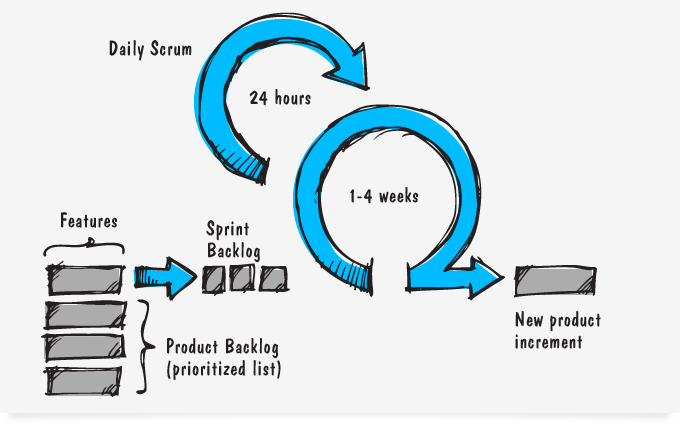
\includegraphics[width=1\textwidth]{imgs/scrum_process_en.png}
\caption{Scrum process}
\label{fig:scrum}
\end{figure}

\subsubsection{Distributed development}

As mentioned earlier, teams will be formed again on January when
Canadian students start their course. After that, three globally
distributed teams will be formatted as show in Figure~\ref{fig:cooperation}.
This means that we will have three scrum teams with 7 or 8 persons in each. Team
formation session will be held in Canada on January and the Finns will
participate in that session using video conferencing system (Google Hangout).
The goal is to build three equally strong scrum teams which all are able to do
end-to-end development.

Teams will be using internet chat, video conferencing and other
communication tools to work with other students who are not in the same site. We
engourange students to try out distributed pair programming so that there would
be Canadian-Finn pairs, but of course this is challenging because of major time
difference.

\begin{figure}[H]
\centering
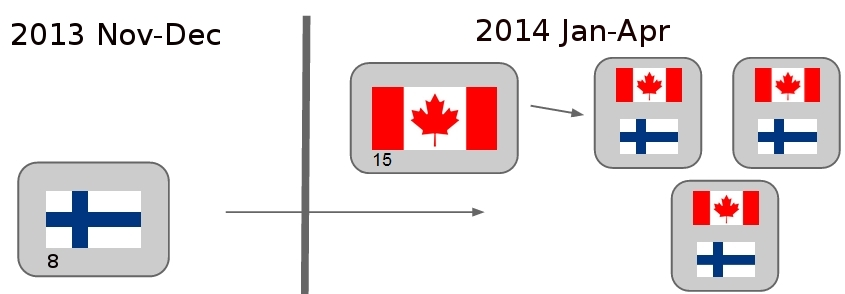
\includegraphics[width=1\textwidth]{imgs/canadacooperation.jpg}
\caption{Canada cooperation}
\label{fig:cooperation}
\end{figure}

\subsubsection{Sprint grooming}

A couple days before the end of a sprint, the project manager grooms the
project backlog with the product owner. Also other team members are allowed to
participate in the meeting if they have time. In this meeting they will
prioritize the project backlog and clarify user stories so that the project
backlog is ready for the sprint planning meeting.

We have agreed with the customer that it's up to product owner to ensure the
project backlog is up to date. Teams have no permission to change the priority
of stories in the project backlog. In addition, the product owner has no
permission to push stories to sprint backlogs, as it's developers' tasks.

\subsubsection{Sprint planning}

Sprint planning session will be divided into two parts. The content of the
sprint planning is presented in Table~\ref{table:Sprintplanning}. The project
manager is responsible for arranging sprint planning sessions.

The sprint planning session will be held using Google Hangout so that The Finns
are located in their team room in Finland and the Canadians are located in their
class room in Vancouver, Canada. In the phase 1, everyone is participated in the
same Hangout, but in the phase 2, teams discuss using separate Hangouts.

\begin{table}[H]
\center
\resizebox{\textwidth}{!}{
\begin{tabular}{|p{1cm}|p{2cm}|p{6cm}|p{3cm}|} 
	
\hline 
\textbf{Part} & \textbf{Duration} & \textbf{Description} & 
\textbf{Participants} \\ 
\hline
1 & 1h & 
The product owner presents the prioritized project backlog, so that the
teams would understand what should be done during a sprint. The product owner is
there for answering any questions the teams would like to ask relating to the
user stories and tasks. In this part top most user stories from the project
backlog are estimated using planning poker method. We don't have cards but we
use hands and fingers to show the estimates. The product owner is leading this
part. Sprint goal is also agreed in this part. When enough stories are
estimated, it's time to start the next phase.
& Product owner, members of each team \\

\hline
2 & 1h & 
After the first phase, teams separate to plan what they can do during the
sprint. The scrum master is responsible for faciliting this phase. The product
owner should be available for teams if they need to ask something. Teams start
with pulling stories from the product backlog to the sprint backlog based on
their knowledge of how much work they are capable of doing during a sprint. When
there are enough stories in the sprint backlog, it's time to plan how the chosen
work will be done during the sprint.

Users stories will be assigned to team members. User stories are split into
tasks and the required time per a task is estimated by a person the task is
assigned to. In this meeting, the team can already start design the system so
that they are able to convert the backlog items into a working software increment.
& Team members \\
\hline
\end{tabular}
}
\caption{The content of a sprint planning}
\label{table:Sprintplanning}
\end{table}

In a sprint planning session (excluding sprint 1), stories are estimated using
story points following the fibonacci scale. Possible story points
are 1, 2, 3, 5, and 10. If the story is estimated to be larger than 10 story
points, it can be seen as an epic and should be split to smaller stories so that
it can be finished during the sprint.

As we have only one product owner and we will have 3 distributed teams, the
planning poker could be challenging to be performed using only hands. In this
reason, we have created
\href{https://docs.google.com/spreadsheet/ccc?key=0Ahu59q_GwtcedFp4dXQzVmFoQWlxandqMkxtdEFiaVE&usp=sharing}{a
planning poker spreadsheet} that can be used for several teams. The idea is that
everyone opens the spreadsheet and type the number under his/her name, but not
press the enter yet. As all estimates has been entered (each cell is gray), the
product owner will count 3, 2, 1 and then everyone press the enter and the story
points are revealed.

The customer said we should not have larger stories than 10 points. We also
agreed that we won't tie story points to any hour estimates. If one story is
estimated to have one story point and an another story is thought to be about
twice as laborious as the first one, it will be given two story points and so
on.

\subsubsection{Sprint review}

Sprint review is held at the end of each sprint. All teams participate in this
meeting. Google Hangout is used to reach everyone. The goal of a sprint review
is to demonstrate to all stakaholders what the teams have accomplished during
the sprint. The meeting should be informal and PowerPoint presentations are
NOT allowed. Teams usually presentes new functionalities they have implemented
and these are discussed with others.

\subsubsection{Documenting}

All course documents need to be public and available for everyone. The course 
personnel and customer should be able to follow the progress of the project by 
seeing our documentation. In addition, the change log of each documents 
documentation should be visible so that changes are easily seen. The official
documentation is written in English.

After a long discussion we deciced that we use Google Docs for course
documentation except the project plan that was started to write using Latex. All
project related documents are stored in Google Drive, to where all stakeholders
have access.

The SE trio is responsible for writing the course documentation. 
Developers can help to write documents based on their interests. Project manager
is responsible for writing the project plan and progress report; the QA is
responsible for writing the QA plan, requirements document, and testing
material; and architect is responsible for documenting the architecture, writing
technical specifications, and user's manual.

\subsubsection{Risk management}

Trio held a risk management session together with one developer. The session was
held in the middle of the first sprint and it took 30 minutes. During the
session several potential risks were identified. When the risks were
identified, we estimated the probability and severity of each risk and discussed a little
bit how to minimize the realization of the risks.

The risk log is maintained regularly by the SE trio. At the end of each sprint
the log is review and updated.

\subsubsection{Time tracking}

The group's time tracking will be applied in Agilefant. The group should follow 
these time tracking practices:
\begin{itemize}
\item Each group member should enter their own hours by themselves in 
Agilefant.
\item Hours are logged directly to the story or more preferably to the task 
after the work is done. 
\item Hours should be logged before leaving the office
\end{itemize}

Agilefant provides burndown charts that are used to follow the project's
progress. Burndown charts tell also whether estimated hours are correlating with
actual hours. That helps the group to shape its task estimation.

Agilefant cannot provide all relevant metrics so the project data is exported to
Excel every Monday. The project manager follows that time is logged in
Agilefant and remind other team members to log hours if needed.

As the group is logging spent effort to the Agilefant, the customer is able to
follow that the project is progressing.

Below are two screenshots of how to log hours to Agilefant. Hours can be entered
by clicking hours number on Spent column or by clicking Spent effort under a
Edit button.

\begin{figure}[H]
\centering
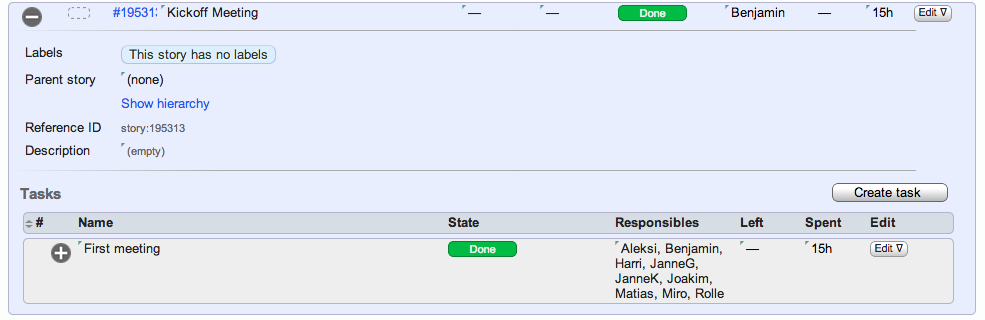
\includegraphics[width=1\textwidth]{imgs/spenteffort1.png}
\caption{Story and task with spent effort}
\label{fig:spenteffort1}
\end{figure}


\begin{figure}[H]
\centering
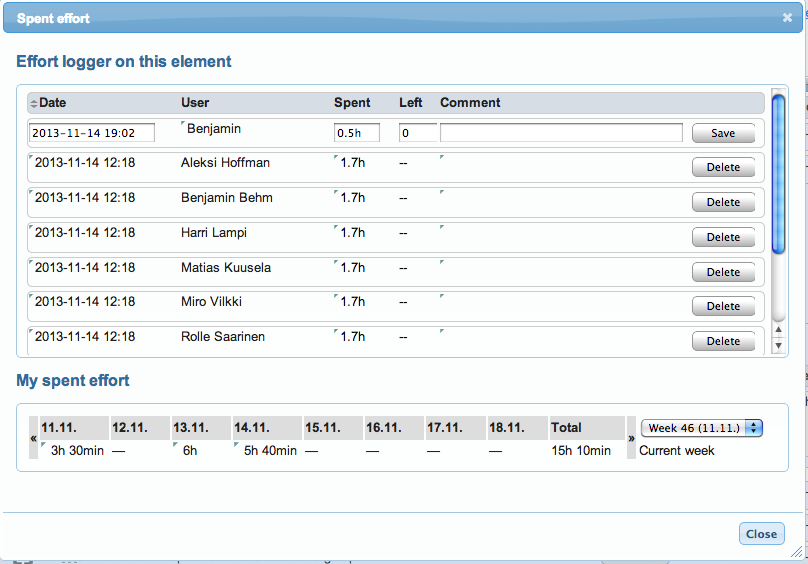
\includegraphics[width=1\textwidth]{imgs/spenteffort2.png}
\caption{Log spent effort}
\label{fig:spenteffort2}
\end{figure}

When the course is over, the Finns will be get credits based on
the hours logged to the Agilefant (+ hours spent on lectures). The view shown in 
Figure~\ref{fig:totalhours} can be found in Agilefant under Timesheets where
user needs to select backlog(s), interval and user(s) to generate the timesheet where used 
hours are listed.

\begin{figure}[H]
\centering
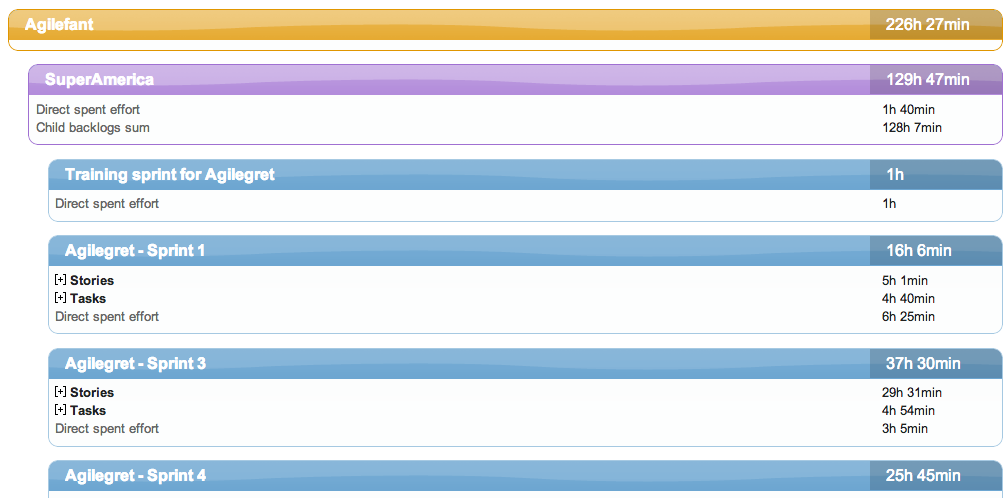
\includegraphics[width=1\textwidth]{imgs/totalhours.png}
\caption{Total used hours}
\label{fig:totalhours}
\end{figure}

\subsubsection{Communication}

Teams will keep a daily scrum meeting during each development day. Before the
Canadians join us, daily scrums will be held in our teamroom. In spring, daily
scrum meetings are held using Google Hangout so that the whole team participates
in them. The daily scrum will be a short, 15-minute time-boxed meeting where
team members synchronize their activities. In this meeting, people will tell, in
turn, three things: What they have done since last daily scrum, what they will
do before the next meeting, and whether there is any obstacles in their way.
Attending to these meeting is important in order to know what is happening
within the team.

Scrum of scrums will be held when three teams have been formed. These meetings
are arranged once or twice per a sprint. The idea is that one member from each team
will keep a short meeting together and share information what each team has been
doing. This helps to solve possible roadblocks that can emerge when several
teams are developing the same application.

We can also try out a practice where a team member attends to other team's daily
scrum to get information about what they are doing. Then the person can share
the information with his/her team.

Flowdock is agreed to be used as a primary communication channel. It allows to
create own communication flows for each team. In addition to team flows,
technical discussions can be separated into own flows, so that all parties who
are interested in the subject can participate in the conversation. These can be
seen as communities of practice. Currently we have separate flows for
documentation, UI and REST.

Google Hangout is proposed to be used for video communication with off-site team
members.

Project manager send a weekly email to all stakeholders to keep them informed
about the progress of the project.

In very urgent situations phone calls or text messaging can be used, but primary
the group is using tools mentioned above.

A public \href{http://tinyurl.com/mobilefant}{Google calendar} is used to share
all events and deadlines of the project. Each team member and other stakeholders
are able to see the calendar and follow our meeting times.

Communication with the customer usually happens face-to-face in our teamroom or
their office.

\subsubsection{Defect tracking}

For defect tracking we are using Github's
\href{https://github.com/soberit/mobilefant/issues}{Issues} application. It is
an easy-to-use tool for keeping track of issues found during the development
process. It allows to assign a person to the issue and define a milestone when
the issue needs to be fixed. It also informs us immediately when new issues are
created. This is one reason why the team wanted to use some real issue tracker
instead of Agilefant. Issues are also automatically posted on our Flowdock
stream from where everyone is able see them.

When a new bug is found, it need to be reported immediately to the issue
tracking system in order to inform everyone else of found issue. The issue can
be closed only when it is fixed and someone else has tested it.

\subsubsection{Version control}

All code should be located in the version control system. Agilefant uses Git
(and Github) so we are also going to use them. Soberit provided us a private
repository. The repository is named as
\href{https://github.com/soberit/mobilefant}{mobilefant}.

We have decided to try out feature branching approach with a single repository.
In feature branching each feature is developed using a separate branch in the
version control system. This means that every time a developer starts a new
feature, he/she will create a new branch for that, and after the feature is
ready, the feature branch will be merged to the main branch. The main branch
should contain only working code, which is verified by compiling the code and
running the test. All tests should pass.

We have to be sure everyone understands how to use Git in order not to mess
the whole repository as everyone has privileges to push anything into master. To
help people to work with Git, we have defined a general
\href{https://docs.google.com/document/d/1wAih0JzkrZ4ySUZ_MO-F8MvGkPXKHicYbG1972Sxo2w/edit?usp=sharing}{git
workflow}. 

To keep the commit message history clear, everyone shouls use the imperative
present tense in commit messages. Furthermore, the commit message should start
with a short summary of changes that can be up to 50 charts long. More
information about development practices can be found
\href{https://docs.google.com/document/d/1Advu6FXwe2axjmO29-fMpw7hbDMeZwJzMF5ad391aBE/edit?usp=sharing}{here}.

\subsubsection{Process improvement}

A retrospective meeting is arranged at the end of each sprint. The goal of
having regular retrospectives is to improve the process and find out the
problems before they cause any bigger problems.

For retrospectives, we are using
\href{http://wirca.soberit.hut.fi/prod/}{ARCA-tool} developed in Aalto
University. It's a tool that helps us to keep better retrospective meetings and
analyze problems more deeply in comparison to the retrospectives kept using
Post-it notes or Spreadsheet. In this way, these meetings can be more
productive, worthwhile and less time will be wasted.

The retrospective meeting is time-boxed to half an hour. We have to have enough
time to sit down and discuss about the past sprint, otherwise there is no reason
to keep this kind of meeting.

The retrospective contains five phases:

\begin{enumerate}
\item First, everyone enters problems to ARCA-tool. (5 min)
\item Second, the entered problems are discussed together. (5 min)
\item Third, everyone enters underlying causes to the problems identified
earlier. (5 min)
\item Fourth, causes are discussed and additional causes are added if needed.
(5 min)
\item Fifth, findings are summarized at the end of the meeting. (10 min)
\end{enumerate}

Figure~\ref{fig:retro1} and Figure~\ref{fig:retro1analysis} show how to use the
ARCA tool and how the data can be analysed. 

\begin{figure}[H]
\centering
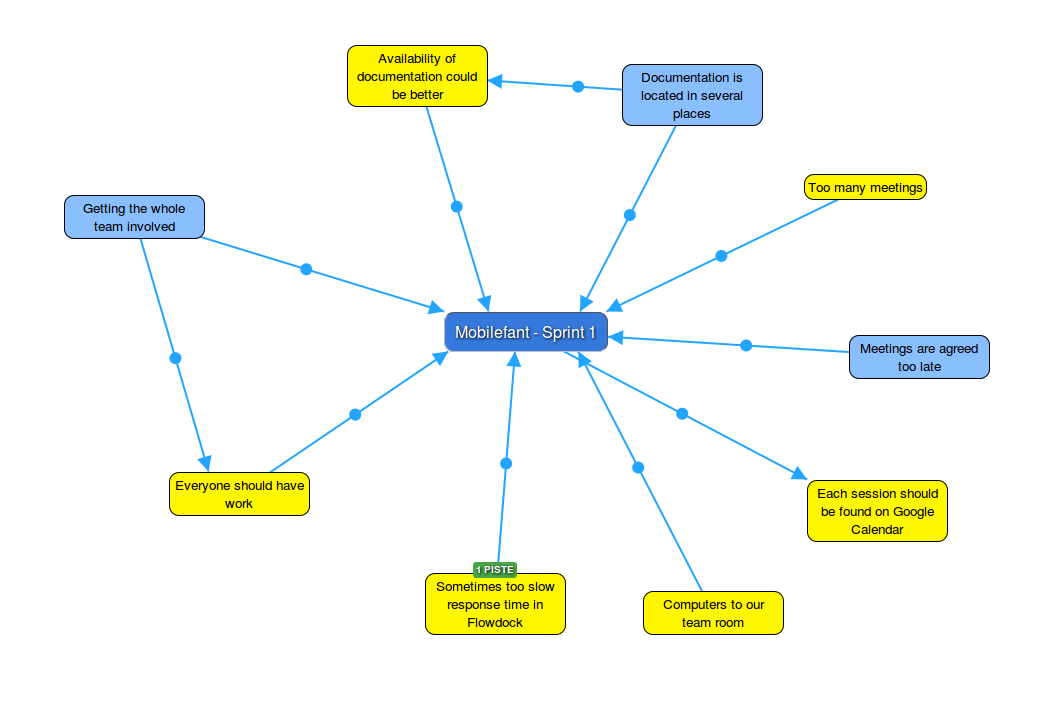
\includegraphics[width=1\textwidth]{imgs/retro-sprint1.png}
\caption{Retrospective - sprint 1}
\label{fig:retro1}
\end{figure}

\begin{figure}[H]
\centering
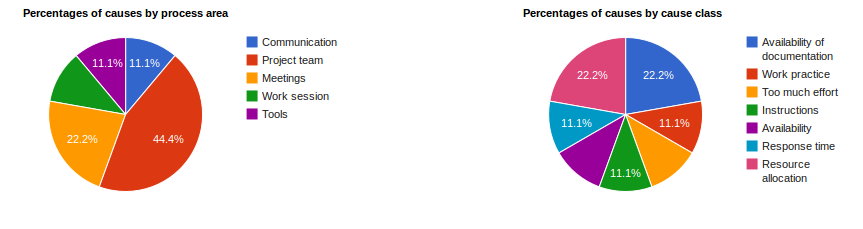
\includegraphics[width=1\textwidth]{imgs/retro-analysis-sprint1.png}
\caption{Retrospective analysis - sprint 1}
\label{fig:retro1analysis}
\end{figure}

\subsubsection{Requirement engineering}

Requirement engineering is up to the SE trio and the produt owner, but other
team members can also participate in the eliciting process. At the beginning of
the project, a requirement engineering session was held with the customer where
high level requirements were defined. In general, the product owner has the
vision of what should be developed and it is up to him to update the project
backlog. The team generates ideas at the same time they are implementing
existing user stories. The ideas are shared with the customer face-to-face or in
Flowdock.

As we are working an agile way, we don't define requirements at a detailed level
at the beginning of the project. But instead, requirements emerge as the
project elapses. The most important requirements are specified and prioritized
in a backlog grooming session at the end of each sprint so that the project backlog
would be up to date in the sprint planning session. All requirements are
collected in Agilefant and it is up to the product owner to keep the project
backlog up to date and prioritized.

Requirements are usually listed in the project backlog in non-user story form to
keep the list clear and readable, but the team together with the product owner
should define the user stories in the description field for each story. This
format helps everyone to capture the who, what and why of a requirement. The
template of a user story is presented below:

\begin{verbatim}
    As a <role>, I want <goal/desire> so that <benefit>.
\end{verbatim}

In a user story, the role and goal/desire are mandatory, but the benefit part is 
optional.

\subsubsection{Design}

Overall architectural design is up to the lead architect, but other teammates
are also allowed to participate in the design process. The customer's lead
developer is actively participating in the architectural planning as he has the
technical view of requirements. As we need not to touch the Agilefant's backend,
we need not to have a detailed view of what is happening in there. We need to
design what technologies are used so that the performance would be good enough and it
follows the techological practices used in the Agilefant's hosted version.

UI design sessions are arranged at the beginning of the project. First, the UI
wireframes are drafted using pencil and paper, but after the drafts are approved
by the customer, they are transferred to digital form using Lucidchart tool.

Two team members were chosen to take the responsible for the UI drafts as they
pointed out they would be willing to do those. More UI wireframes are drawn as
they are needed.

\subsubsection{Coding standards}

To produce clean and understandable code, we use coding standards defined by
\href{http://code.google.com/p/google-styleguide/}{Google}. Style guides for
\href{http://google-styleguide.googlecode.com/svn/trunk/htmlcssguide.xml}{HTML,
CSS} and
\href{http://google-styleguide.googlecode.com/svn/trunk/javascriptguide.xml}{JavaScipt} are the most important ones everyone should be familiar with.

\subsection{Quality assurance plan}

Quality assurance plan will be written later by QA.

\section{Phasing}

Tasks are not listed in this project plan, as they are listed and maintained in 
\href{https://cloud.agilefant.com/dev/}{Agilefant}.

As presented in Scrum, a product owner is responsible for keeping up the
project backlog. The students pull stories from the project backlog to sprint
backlogs which are listed below:

\begin{itemize}
  \item
  \href{https://cloud.agilefant.com/dev/ROIteration.action?readonlyToken=656371244996018241588558287820343266020}{Sprint
  1}
  \item
  \href{https://cloud.agilefant.com/dev/ROIteration.action?readonlyToken=807072238002616723743205864538724805102}{Sprint
  2}
\end{itemize}

\subsection{Schedule}

The spring's schedule is still an open question as we don't know how we are
going to organize the third sprint in Canada and when the fourth sprint should
start. We need to discuss about this with our mentor and the Canadian professor.
There are three optional schedules that are presented below. In the first one we
would hold the sprint planning sessions on Mondays, while in the others it is on
Thursdays. In the second one, we have only sprints of two weeks after the
Christmas, excluding the sprint 3. The last one takes into account that we have
an exam week here in Finland on week 8, so the sprint 6 would be 3 weeks long.

Project manager and QA are flying to Canada with the customer and mentor on
8.1.2014 - 20.1.2014 (preliminary days). Their task is to help Canadian students
to get in to the project by teaching them what Agilefant is and what processes
we are using. This is kind of kickoff session for them.

\paragraph{Option 1}

\begin{verbatim}
Sprint 1 (13.11.2013 - 27.11.2013)
Sprint 2 (27.11.2013 - 11.12.2013)
Christmas vacation
Sprint 3 (7.1.2014 - 20.1.2014)
Sprint 4 (20.1.2014 - 3.2.2014)
Sprint 5 (3.2.2014 - 24.2.2014)
Sprint 6 (24.2.2014 - 10.3.2014)
Sprint 7 (10.3.2014 - 24.3.2014)
Sprint 8 (24.3.2014 - 9.4.2014) 
\end{verbatim}

\paragraph{Option 2}

\begin{verbatim}
Sprint 1 (13.11.2013 - 27.11.2013)
Sprint 2 (27.11.2013 - 11.12.2013)
Christmas vacation
Sprint 3 (7.1.2014 - 16.1.2014)
Sprint 4 (16.1.2014 - 30.1.2014)
Sprint 5 (30.1.2014 - 13.2.2014)
Sprint 6 (13.2.2014 - 27.2.2014) (An exam week)
Sprint 7 (27.2.2014 - 13.3.2014)
Sprint 8 (13.3.2014 - 27.3.2014)
Sprint 9 (27.3.2014 - 9.4.2014)
\end{verbatim}

\paragraph{Option 3}

\begin{verbatim}
Sprint 1 (13.11.2013 - 27.11.2013)
Sprint 2 (27.11.2013 - 11.12.2013)
Christmas vacation
Sprint 3 (7.1.2014 - 16.1.2014)
Sprint 4 (16.1.2014 - 30.1.2014)
Sprint 5 (30.1.2014 - 13.2.2014)
Sprint 6 (13.2.2014 - 6.3.2014) (3 weeks because of an exam week)
Sprint 7 (6.3.2014 - 20.3.2014)
Sprint 8 (20.3.2014 - 3.4.2014)
Sprint 9 (3.4.2014 - 9.4.2014) (Wrapping up) 
\end{verbatim}

Table~\ref{table:dates} presents project related dates that are important to
remember. It does not contain upcoming sprint changes or other times relating to
sprints as our schedule is not confirmed yet.

\begin{table}[H]
\center
\begin{tabular}{|p{2cm}|p{3.8cm}|p{4.1cm}|} 
	
\hline 
\textbf{Date} & \textbf{Time} & \textbf{Event}\\ 
\hline
13.11.2013 &  &  Sprint 1 starts \\
\hline
26.11.2013 & klo 14:15-16 &  EES: Project managers \\
\hline
26.11.2013 & klo 16:15-18 &  EES: QA managers - req. engineering \\
\hline
27.11.2013 &  &  Sprint 2 starts \\
\hline
09.12.2013 & klo 13 &  DL: All documents \\
\hline
11.12.2013 & klo 11-12 & Project review (PP) \\
\hline
12.12.2013 - 06.01.2014 &  &  Christmas vacation \\
\hline
08.01.2014 - 20.01.2014 &  &  PM, QA, Customer and Mentor in Canada \\
\hline
28.01.2013 & klo 14:15-16 &  EES: Architects/Developers \\
\hline
28.01.2013 & klo 16:15-18 & EES: QA managers - quality \\
\hline
29.01.2014 & klo 16-18 &  EES: Project managers \\
\hline
17.02.2014 & klo 13 &  DL: All documents \\
\hline
19.02.2014 & klo 11-12 & Project review (I1) \\
\hline
31.03.2014 & klo 13:00 &  DL: Delivery of the finalized system to the peer
group\\
\hline
01.04.2014 & klo 14:15-16 & EES: Architects/Developers \\
\hline
01.04.2014 & klo 16.15-18 & EES: QA managers  \\
\hline
02.04.2014 & klo 16-18 &  EES: Project managers\\
\hline
03.04.2014 & klo 13 & DL: Delivery of the peer testing results to the peer group
\\
\hline
07.04.2014 & klo 13 & DL: Delivery of all documents \\
\hline
08.04.2014 - 09.04.2014 &  & Project review (I2) \\
\hline
\end{tabular} 
\caption{Important dates}
\label{table:dates}
\end{table}

\subsection{Sprint 1 Plan}

\paragraph{Sprint goal}~\\
Everyone understands the domain of the project and customer collaboration has
been started. \checked

\paragraph{General goals}~
\begin{itemize}
  \item To understand Agilefant's vision \checked
  \item To have the main requirements from the Customer \checked
  \item To understand the used process \checked
  \item To understand the domain \checked
  \item To have a draft of UI using wireframes \checked
  \item To know required technologies \checked
  \item To know tools that are going to be used \checked
  \item Working place ready at A243 with a couple of work stations \checked
\end{itemize}

\subsection{Sprint 2 Plan}

\paragraph{Sprint goal}~\\
To develop version 0.1 with a simple task queue view.

\paragraph{General goals}~
\begin{itemize}
  \item To have the development environment set up to everyone \checked
  \item To have everyone working with the code \checked
  \item To have the code base ready
  \item To have the high-level architecture design ready
  \item To have the wireframes ready \checked
  \item To identify risks in the project \checked
  \item To have an initial architecture ready \checked
\end{itemize}

\paragraph{Deliverables}~
\begin{itemize}
  \item Project plan (no QA plan) \checked
  \item Progress report slides \checked
  \item Contract (one per a group) \checked
  \item Requirements document (except details of requirements) \checked
\end{itemize}

\subsection{Sprint 3 Plan}

\paragraph{General goals}~
\begin{itemize}
  \item To get to know the Canadian students
  \item To familiarize Canadian students to the practices and processes
  \item To form three distributed teams
\end{itemize}

\paragraph{Deliverables of Implementation 1 phase}~
\begin{itemize}
  \item Project plan
  \item Progress report
  \item Requirements document 
  \item Technical specification (at least the general architecture)
  \item QA plan 
  \item Test cases and test log
\end{itemize}

\paragraph{Deliverables of Implementation 2 phase}~
\begin{itemize}
  \item Project plan
  \item Project review slides
  \item Final report
  \item Requirements document
  \item Technical specification
  \item User's manual 
  \item Peer test materials to peer group
  \item Peer test results to peer group
  \item QA plan
  \item Test cases and test log
  \item Peer test session charters with logs (own and peer group's)
\end{itemize}

\section{Risk log}

\begin{table}[H]
\center
\resizebox{\textwidth}{!}{
\begin{tabular}{|p{0.5cm}|p{3cm}|p{1cm}|p{1cm}|p{4cm}|p{4cm}|p{1.5cm}|} 
	
\hline % The line on top of the table
\textbf{ID} & \textbf{Risk} & \textbf{Prob.} & \textbf{Sev.} & \textbf{Effects} 
& \textbf{Controlling actions} & \textbf{Resp.} \\ 
\hline

1 &
A developer quits in the middle of the project. &
2 &
3 & 
Some knowledge is lost. Project scope must be decreased. &
Taking care of good team spirit. Using pair programming. &
PM / team \\
\hline

2 & 
Adapting with Scrum practices is harder than expected. & 
2 & 
2 & 
Productivity is lower than assumed and stories cannot be finished on time. & 
Providing enough training. & 
PM \\
\hline

3 &
The team could not build a code base that is wide enough to divide development 
tasks among three teams on January. &
3 &
3 &
All developers cannot start development right away, but need to wait until the 
code base is ready. The project scope must be decreased. &
Architectural design needs to be started as soon as possible. Team members
should start coding small features as soon as possible to get familiar with
technologies.
& AR \\
\hline

4 &
The customer has to leave the CS-building on January, 2014. &
2 &
3 &
Getting feedback takes longer and the amount of face-to-face meetings decreases. 
&
To generate a backup plan of how stay contacted with the customer. &
PM / Customer \\
\hline

5 &
Merge conflicts in Git when all have privileges to push code to master. &
3 &
3 &
Lots of effort have to put to resolve the problems. &
Git training should be provided to everyone if needed. &
PM \\
\hline

6 &
Non-experienced users mess the Git repository. &
3 &
3 &
Lots of effort have to put to resolve the problems. &
Git training should be provided to everyone if needed. &
PM \\
\hline

7 &
Major changes in requirements. &
1 &
3 &
The outcome of the project will suffer. &
We should collaborate actively with the customer to stay informed about
requirements. & 
Customer / teams \\
\hline

8 &
Communication with off-site team members won't work as supposed. &
2 &
3 &
Stories are not finished on time. People won't know what others are doing. &
Scrum master should observe that good communication practices are followed. &
SM \\
\hline

9 &
A team divides to sub-teams. &
3 &
3 &
Team's efficiency decreases and the team spirit suffers. &
Scrum master should observe procedures within a team. &
SM \\
\hline

10 &
REST API is not working properly. &
2 &
3 &
All data is not available. Effort should be allocated to develop the REST API. &
Customer should put effort to ensure that the REST API is working properly.
& Customer, AR \\
\hline

11 &
Lack of proper testing devices. &
3 &
2 &
Correct behaviour of the application cannot be tested using wide range of real
devices.
& Using our own devices and different emulators. & 
Customer \\
\hline

12 &
The Finns' hours run out before the end of the course. &
3 &
3 &
Cooperation with Canadian students is harder. &
Hour usage need to be followed. Developers with lower amount of credits
work less during the fall. &
PM \\
\hline

13 &
Chosen technologies are not suitable for our needs. & 
1 &
3 &
Major changes need to be done and project scope will be decreased. &
Architecture should be well designed together with the customer at the
beginning of the project. &
AR \\
\hline


\end{tabular} 
}
\caption{A risk log (Probability: 1=lowest, 3=highest, Severity: 1= lowest, 
3=highest)}
\label{table:Risklog}
\end{table}

\subsection{Materialized risks}

\paragraph{Risk 1}~

One developer quit during the first sprint as he found out he wouldn't be able
to participate in the project as required. We discussed about it with the mentor
and the team, and we decided that he will take the course later again.

